\documentclass[pageno]{jpaper}

%replace XXX with the submission number you are given from the ASPLOS submission site.
\newcommand{\asplossubmissionnumber}{684}

\usepackage[normalem]{ulem}

\usepackage{fancyhdr}

\pagestyle{fancy}
\fancyhf{}
\rhead{}
\lhead{A Study of Energy Efficiency in Operating Systems}
\rfoot{Page \thepage}
\begin{document}

\title{A Study of Energy Efficiency in Operating Systems \\ \textbf{Appendix}}

\date{}

%\maketitle

%\thispagestyle{empty}

%\section{Detail hardware parameter per Applications}
%We find that using RAPL at a maximum of 135\watt or a minimum of 55\watt produces no major performance or energy saving impact. We attribute this to the fact that RAPL power limiting is applied to the entire processor package, and hence a network-intense application, such as netpipe, running on a single core does not use enough power to warrant power limiting features to come into play.

%\begin{itemize}
%    \item \textbf{netpipe} and \textbf{nodejs}: For interrupt-delay, we use 15 values that range between 0 and 100 $\micro$s in Linux. It turns out that our library OS needs a minimum of six $\micro$s due to its device driver implementation which requires receive-side coalescing to handle large packet receives. For DVFS, we select nine values between \texttt{0xC00} and \texttt{0x1D00}.
%    \item \textbf{memcached} and \textbf{memcached-silo}: For interrupt-delay, we use values of 50 $\micro$s, 100 $\micro$s, 200 $\micro$s, 300 $\micro$s, and 400 $\micro$s. For DVFS, we select the same nine values between \texttt{0xC00} and \texttt{0x1D00} as above. For RAPL, we use four values of 135\watt, 95\watt, 75\watt, and 55\watt.
%\end{itemize}
%\subsection{Data collection overview}
%\begin{center}
The above plots are examples of visualizations that summarize our full data sets.  Here we are visualizing all the EDP data form a single NetPipe study at one message size.  To the right we see the tuning curves and EDP summaries.  Such visualizations exist for our entire data sets which is in excess of 2T of data and documents more than 5000 individual experiments including a Silo-memcached study not documented in this paper.
%\end{center}

\begin{figure}
	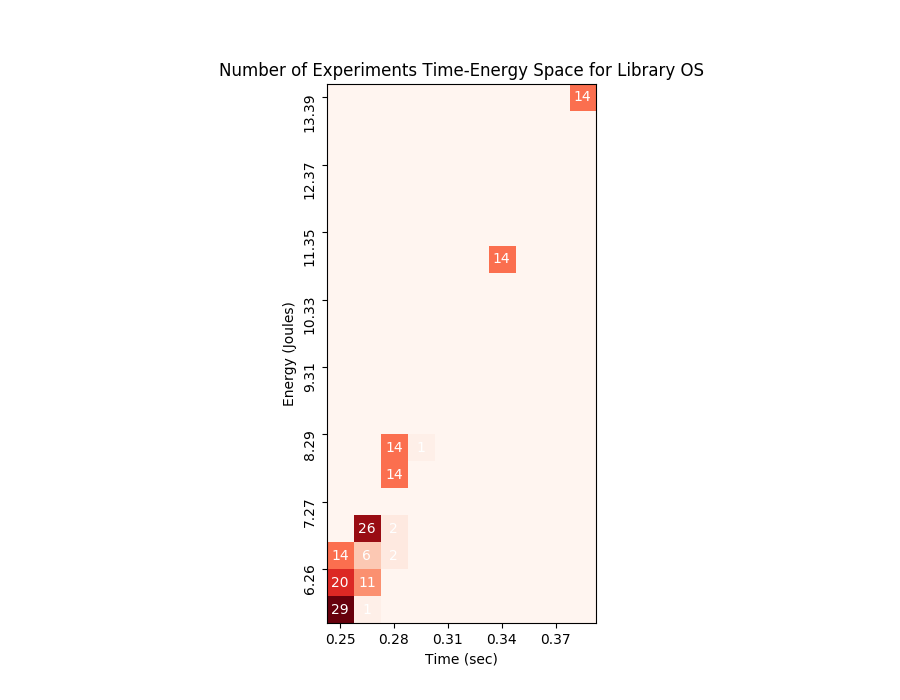
\includegraphics[width=\columnwidth]{asplos2021_figures/plots3d_netpipe_heatmap_ebbrt_tuned.png}
	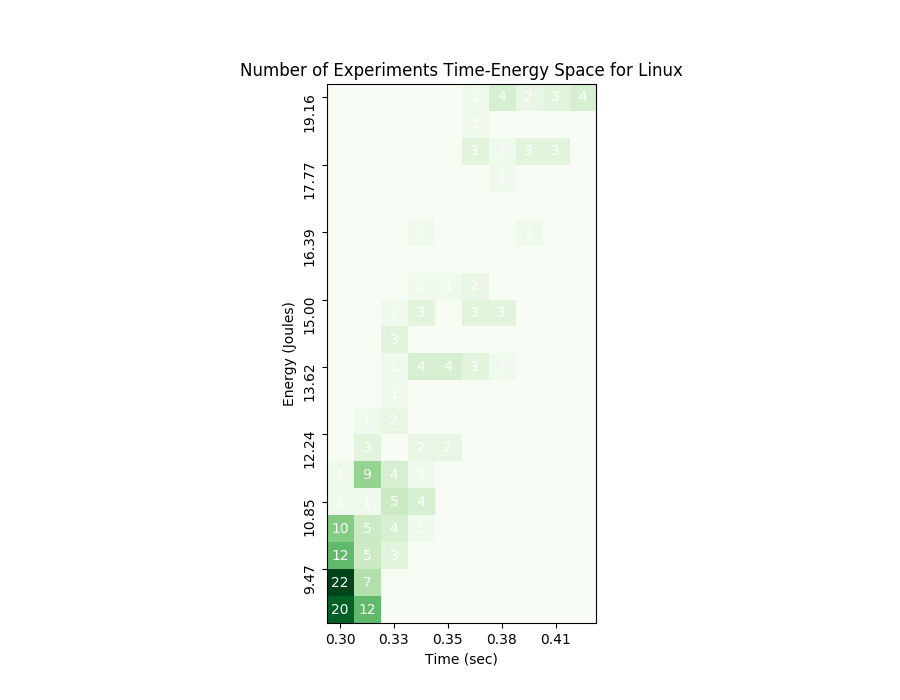
\includegraphics[width=\columnwidth]{asplos2021_figures/plots3d_netpipe_heatmap_linux_tuned.png}
\end{figure}

\begin{figure}
	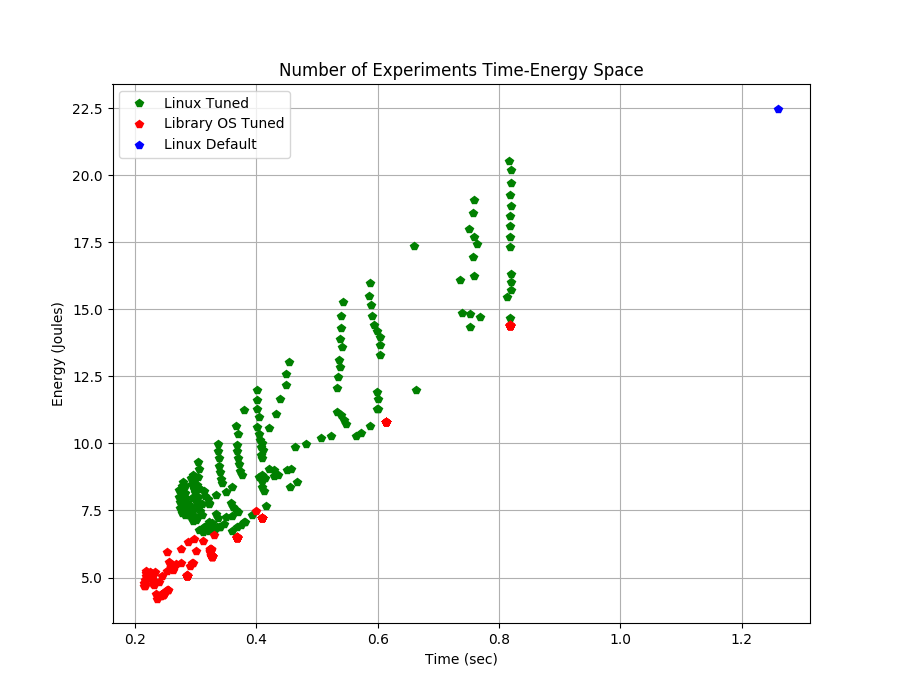
\includegraphics[width=\columnwidth]{asplos2021_figures/plots3d_netpipe_scatter_points.png}
	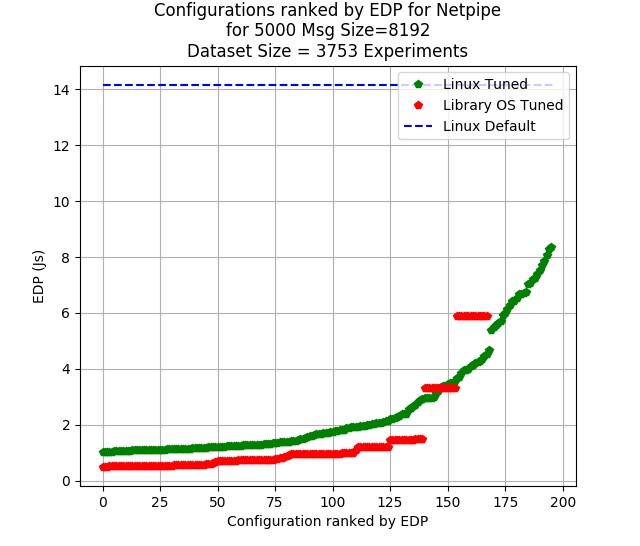
\includegraphics[width=\columnwidth]{asplos2021_figures/plots3d_ranked_netpipe_msg8192.png}
\end{figure}

\textbf{Memcached-silo}~\cite{mcdsilo} is an addition on top of the normal memcached protocol used to reflect a more complex workload which includes a combination of latency sensitive network traffic and compute and memory intensive TPC-C style transaction processing. We ported memcached-silo, that was developed by previous work done on building scalable $\micro$s-scale in-memory compute servers~\cite{zygos}, to the library OS. The configuration and SLA of memcached-silo follows from that of memcached (listed above). Given its computationally heavier nature, we only needed two 16-core server nodes at 16 connections per core to saturate our memcached-silo server.
\begin{figure}
	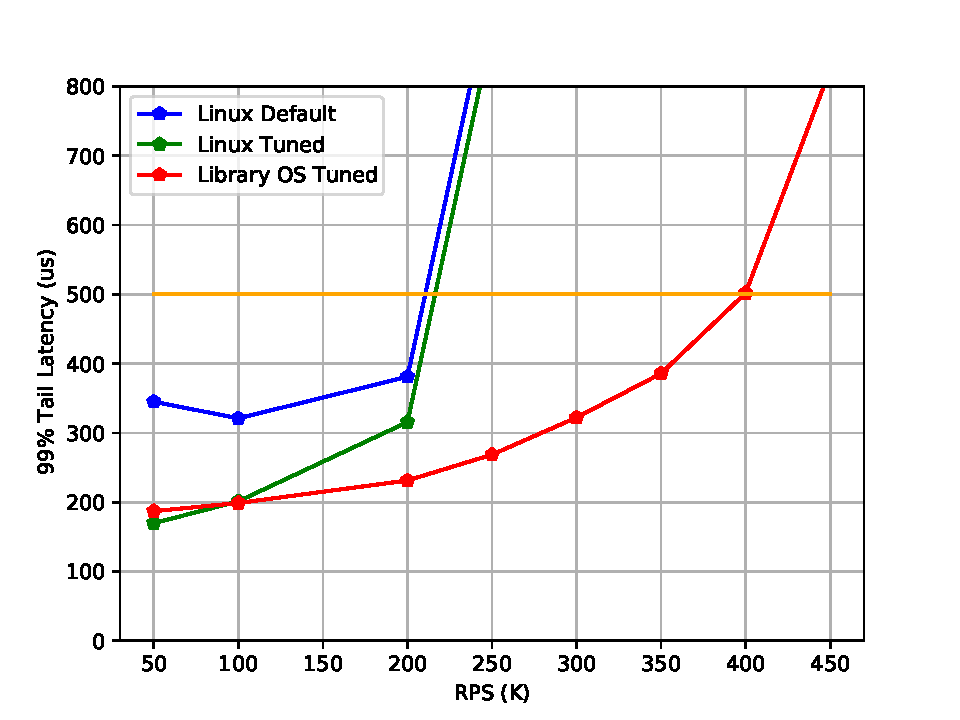
\includegraphics[width=\columnwidth]{asplos2021_figures/mcdsilo_sla.pdf}
	\caption{Memcached-silo QPS results with 99\% tail latency < 500 us}
\end{figure}
\begin{figure}
	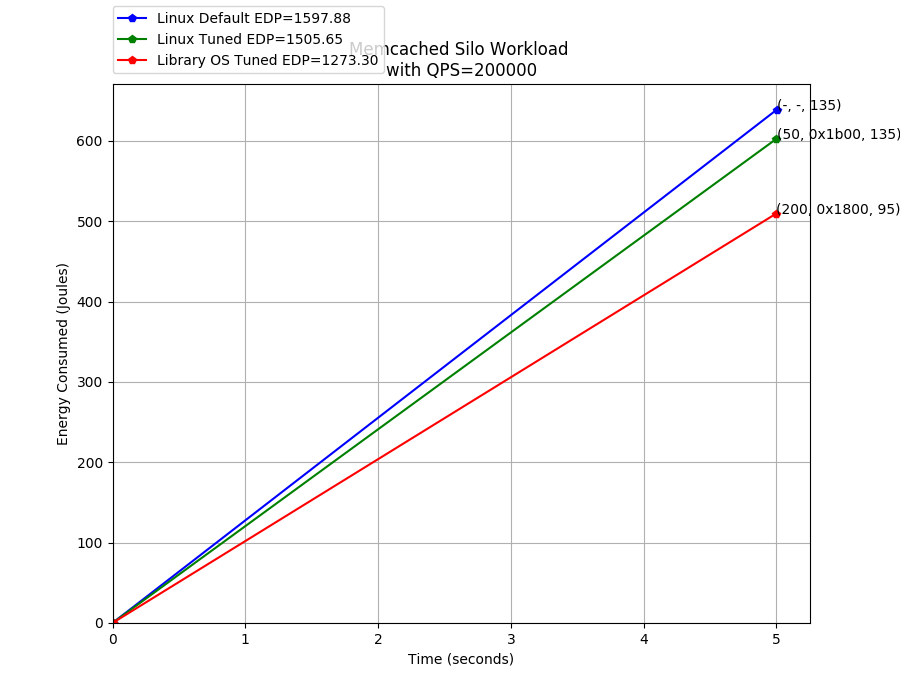
\includegraphics[width=\columnwidth]{asplos2021_figures/mcdsilo_edp_aggregated_qps200000.png}
	\caption{Memcached-silo EDP plots}
\end{figure}
\begin{figure}
	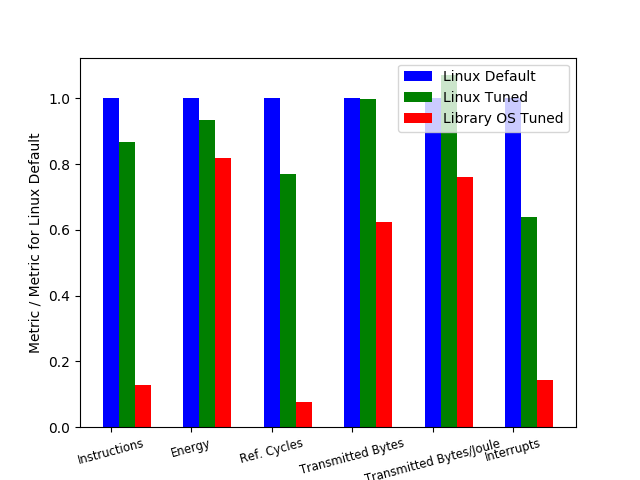
\includegraphics[width=\columnwidth]{asplos2021_figures/mcdsilo_combined_barplot_QPS200000.png}
	\caption{Memcched-silo aggregated data plots of hardware statistics}
\end{figure}
\begin{figure}
	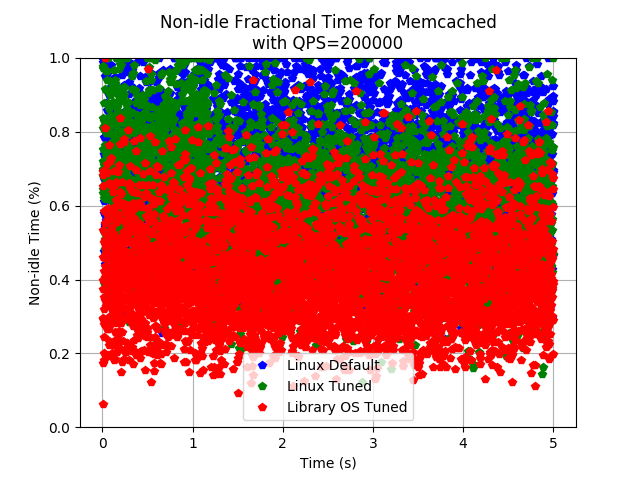
\includegraphics[width=\columnwidth]{asplos2021_figures/mcdsilo_nonidle_QPS200000.png}
	\caption{Memcached-silo nonidle plots}
\end{figure}
%\section{Memcached-silo}  
%

%\pagebreak
\bibliographystyle{plain}
\bibliography{references}


\end{document}